\documentclass[a4paper]{article}
\usepackage[utf8]{inputenc}
\usepackage[italian]{babel}
\usepackage[T1]{fontenc}
\usepackage{graphicx}
\usepackage{amsmath}
\usepackage{amssymb}
\usepackage{caption}
\usepackage[output-decimal-marker={,}]{siunitx}
\usepackage{booktabs}
\usepackage{subfig}
\usepackage{float}
\usepackage{geometry}
\usepackage{multicol}
\usepackage{listings}
\geometry{
	a4paper,
	total={170mm,257mm},
	left=20mm,
	top=20mm,
}

\title{Visibility Curve of an Object}
\author{Alessandro Lattanzi}
\date{\today}

\begin{document}
\maketitle
	
	\section{Introduction}
		This small computer program was built in order to compute the visibility curve of a sky object on a given day.\\
		The program outputs the object's rise, culmination and set times, minimum airmass, Alt. and Az. plots, the Sun's rise and set time and the beginning and end time for civil and astronomical twilight.\\
		
		The resulting curves were confronted with other similar tools available online with good results.
	\vspace{0.035\textheight}
	\begin{multicols}{2}
	\section{Details on the Algorithm}
		\underline{\textbf{NB:}} All non-time quantities are expressed in degrees\\
		\indent\indent where not otherwise specified.\\
		
		The calculation follows the algorithm shown in Ch. 15 of "Astronomical Algorithms" with some details from "Explanatory Supplement to the Astronomical Almanac, 3rd Edition" and from the USNO.\\
		
		The needed information is: Date of Observation, Object ICRS coordinates ($\alpha$, $\delta$), Observer latitude ($\phi$) taken as positive in the northern hemisphere and negative in the southern, longitude ($L$) taken as positive eastward from the prime meridian and negative westward, and height above mean sea level ($H_{msl}$).\\
		
		First the Greenwich Apparent Sidereal Time at $0^h$ UT ($\Theta_0$) on the day of the observation is computed.\\
		For this calculation an algorithm from USNO is used.\\
		In the approximation $JD_{TT} \sim JD_{UT} \doteq JD$, at $0^h$ let $D = JD - 2451545.0$ be the number of days since Jan 1st 2000 at 12:00 and let $T = D/36525$ be the number of centuries since the year 2000.\\
		The Greenwich Mean Sidereal Time (GMST) is given by
		\begin{multline*}
			GMST = (6.697375 + 0.065709824279 D+\\ + 0.0000258 T^2) \% 24
		\end{multline*}
		where "$\%$" is the modulo operator.\\
		A correction for the nutation in right ascension is needed to get the GAST:
		\begin{equation}
			\Theta_0 = (GMST + \Delta\psi \cos(\epsilon))\frac{360}{24}
		\end{equation}
		where $\Delta\psi \simeq -0.000319 \sin(\Omega) - 0.000024 \sin(2L_S)$ 
		is the nutation in longitude in hours,\\ $\Omega = 125.04 - 0.052954 D$ is the longitude of the ascending node of the Moon, $L_S = 280.47 + 0.98565 D$ is the mean longitude of the Sun and \\$\epsilon = 23.4393 - 0.0000004 D$ is the obliquity.\\
		
		Then the apparent RA and Dec of the body\footnote{"Apparent" coordinates are "True Equator True Equinox" coordinates} at $0^h$ Dynamical Time\footnote{"Dynamical Time" is used in the book as an abbreviated form of "Barycentric/Terrestrial Dynamical Time", TDT is needed and henceforth abbreviated TT for "Terrestrial Time"} on day D-1, D and D+1 are needed, all expressed in degrees. These sets of coordinates will henceforth be indicated as ($\alpha_i$,$\delta_i$) with $i = 1,2,3$.\\
		To convert from ICRS coordinates to the needed coordinates the python package Astropy is used.\\
		
		A first guess on the rise ($m_1$), culmination ($m_0$) and set ($m_2$) times, expressed as fractions of day, is given by:
		\begin{align}
			m_0 &= \frac{\alpha_2 - L - \Theta_0}{360}\\
			m_1 &= m_0 - \frac{H_0}{360}\\
			m_2 &= m_0 + \frac{H_0}{360}
		\end{align}
		where $H_0$ is the hour angle of the body such that
		\begin{equation*}
			cos(H_0) = \frac{\sin(h_0)-\sin(\phi)\sin(\delta_2)}{\cos(\phi)\cos(\delta_2)}
		\end{equation*}
		with $h_0$ being the geometric altitude of the body center at the time of apparent rising or setting.\\
		If $\cos(H_0) > 1$ the object is always under the horizon on the day of the observation, similarly if $\cos(H_0) < -1$ the object is always visible.\\
		The value of $h_0$ varies depending on the observed body ($-34/60^{\circ}$ for a star/planet, $-50/60^{\circ}$ for the Sun, $-6^{\circ}$ for civil twilight, $-18^{\circ}$ for astronomical twilight) and includes a correction for the observer's height above MSL ($-0.0353\sqrt{H_{msl}}$).\\
		
		An iterative correction on the three fractions is needed to get more precise estimates.\\
		First the time difference between Terrestrial Time and UT is needed: $\Delta T = TT - UT$. This calculation follows from empirical formulae.\\
		The following procedure is applied separately on each of the three m.\\
		First the sidereal time at Greenwich is computed from $\theta_0 = \Theta_0 + 360.985647m$.\\
		Then an estimate for the apparent RA and Dec at the day fraction is computed from
		\begin{align}
			\alpha(m) &= \alpha_2 + \frac{n}{2}(a + b + nc)\\
			\delta(m) &= \delta_2 + \frac{n}{2}(a + b + nc)
		\end{align}
		where $n = m + \Delta T/86400$, $a = \alpha_2 - \alpha1$, $b = \alpha_3 - \alpha2$, $c = b - a$ (and similar formulae for $\delta(m)$).\\
		This estimate is needed to compute the local hour angle of the body $H = \theta_0 + L - \alpha(m)$ from which one derives the body Azimuth and Altitude angles as:
		\begin{equation}
			\tan(A(m)) = \frac{\sin(H)}{\cos(H)\sin(\phi)-\tan(\delta(m))\cos(\phi)}
		\end{equation}
		\begin{multline}
			\sin(h(m)) = \sin(\phi)\sin(\delta(m)) + \\+\cos(\phi)\cos(\delta(m))\cos(H)
		\end{multline}
		\vfill\null
		\columnbreak
		The correction is then given by
		\begin{equation}
			m = m + \Delta m
		\end{equation}
		with
		\begin{align}
			\Delta m &= - H/360 \qquad\qquad\qquad\quad\quad\quad\textrm{ for }m_0\\
			\Delta m &= \frac{h - h_0}{360\cos(\delta(m))\cos(\phi)\sin(H)} \quad\textrm{for }m_{1/2}
		\end{align}
		The iterative procedure stops when the corrections are small.\\
		
		At the end of the procedure the three m values are converted to times in order to be displayed.\\
		The calculation from the estimate of $\theta_0$ to that of $A(m)$ and $h(m)$ is repeated at steps of m between $m_1$ and $m_2$ in order to plot the Alt/Az curves.
	\end{multicols}
	\vspace{0.4\textheight}
	\section{References}
		\begin{itemize}
			\item Meeus J., "Astronomical Algorithms" (Willmann-Bell)
			\item Urban S. E., Seidelmann P. K., "Explanatory Supplement to the Astronomical Almanac, 3rd Edition", (University Science Books)
			\item USNO, https://aa.usno.navy.mil/
		\end{itemize}

	\newpage
	\section{Software Usage}
		The user can choose at the beginning ("Interactivity (y/n): >>y") if he wants to enter all parameters such as observation date, object coordinates and location, otherwise ("Interactivity (y/n): >>n") the current day, a standard object (M31) and location (Massa, MS) are chosen.\\
		
		\begin{scriptsize}
		\begin{verbatim}
			[Output]
			Interactivity (y/n): >>y
			Date of Observation:
			        Year: >>2023
			        Month: >>9
			        Day: >>19
			Object ICRS Coordinates:
			        Object RA [deg]: >>101.28715533
			        Object Dec [deg]: >>-16.71611586
			Observer Coordinates:
			        For Latitude + in the Northern Hemisphere, - in the Southern
			        For Longitude + westwards from Prime Meridian, - eastwards
			        Observer Latitude [deg]: >>44.007947
			        Observer Longitude [deg]: >>10.099098
			        Observer Height MSL [m]: >>0
			
			Sun:
			        Astro Twilight End:      2023-09-19 03:24:50 [UTC]
			        Civil Twilight End:      2023-09-19 04:33:55 [UTC]
			        Rising:                  2023-09-19 05:02:49 [UTC]       Az. from North 86.99 [deg]
			        Transit:                 2023-09-19 11:13:29 [UTC]       Az. from North 180.00 [deg]
			        Setting:                 2023-09-19 17:23:23 [UTC]       Az. from North 272.73 [deg]
			        Civil Twilight Start:    2023-09-19 17:52:12 [UTC]
			        Astro Twilight Start:    2023-09-19 19:01:01 [UTC]
			
			Object:
			        Rising:          2023-09-19 01:19:07 [UTC]       Alt. -0.57 [deg]        Az. from North 113.01 [deg]
			        Transit:         2023-09-19 06:14:12 [UTC]       Alt. 29.26 [deg]        Az. from North 180.00 [deg]     Airmass 2.046
			        Setting:         2023-09-19 11:09:16 [UTC]       Alt. -0.57 [deg]        Az. from North 246.99 [deg]
		\end{verbatim}
		\end{scriptsize}
		
		\begin{figure}[h!]
			\centering
			\begin{minipage}{0.48\textwidth}
				\centering
				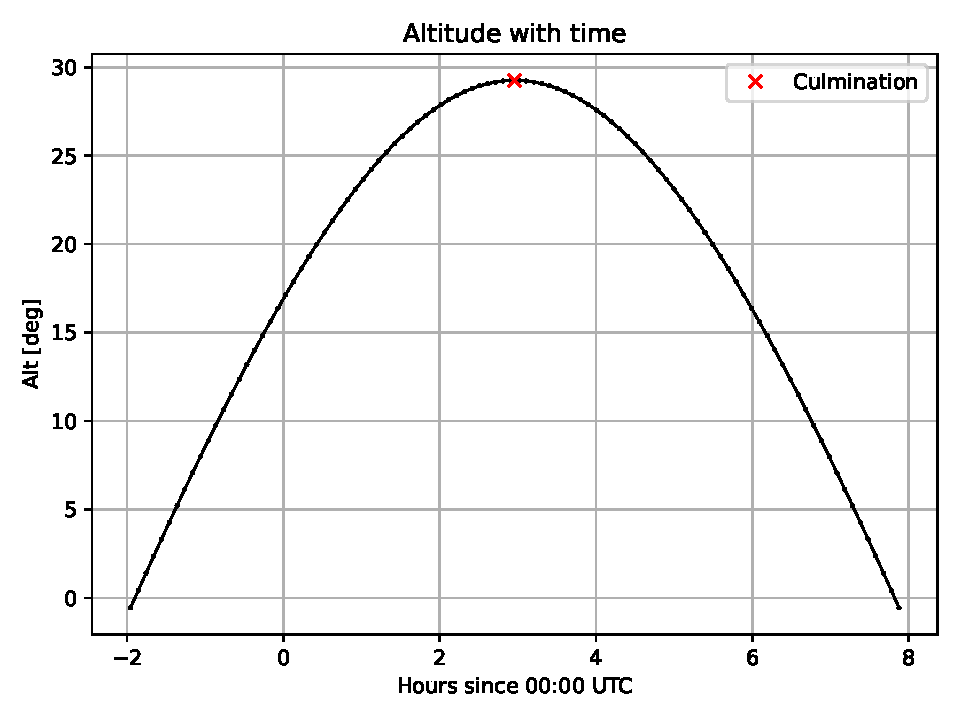
\includegraphics[width=0.95\textwidth]{Alt.pdf}
			\end{minipage}\hfill
			\begin{minipage}{0.48\textwidth}
				\centering
				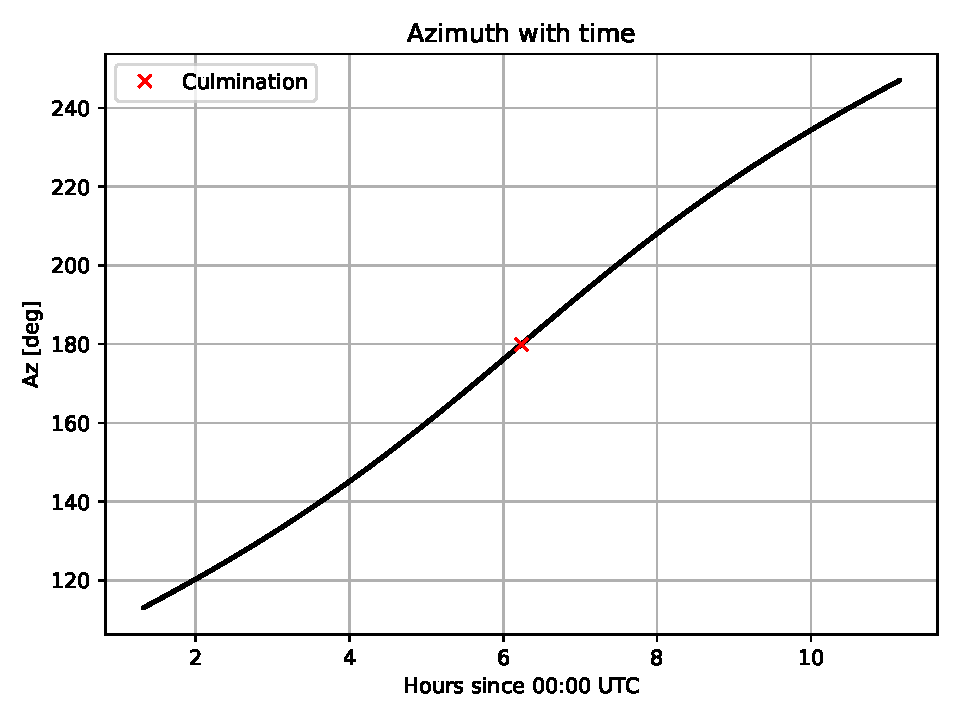
\includegraphics[width=0.95\textwidth]{Az.pdf}
			\end{minipage}
		\end{figure}

		
\end{document}